
\subsubsection{3.1 Problem Formulation}

Let $\mathcal{Z} = \{(W_i, y_i^{\text{gap}}, y_i^{\text{acc}})\}_{i=1}^N$ be a model zoo where $W_i$
denotes the full weight tensor of model $i, y_i^{\text{acc}} = $ test accuracy, and
$y_i^{\text{gap}} = $ train\_acc $-$ test\_acc (generalization gap at convergence). We consider four
encoder functions $f_\theta : W \mapsto \hat{y} \in \mathbb{R}$ and evaluate Spearman rank correlation
$\rho(\hat{y}, y)$ on a held-out test split. The dual-target design evaluates each encoder on both
$y^{\text{gap}}$ and $y^{\text{acc}}$ under identical conditions.

Spearman rank correlation is used as the primary metric because practitioners care about relative
ranking among models (which is least overfit?) rather than absolute gap magnitude, and because
Spearman is robust to output scale mismatches between encoders.

\subsubsection{3.2 A1 Prerequisite Audit}

Before any encoder training, we verify that gap and test accuracy are not trivially collinear in the zoo:

$$\rho_{\text{A1}} = |\text{Spearman}(\text{gap}, -\text{test\_acc})| < 0.95$$

If A1 fails (collinearity), the dual-target experiment conflates two versions of the same task. We measure
$\rho_{\text{A1}} = -0.142$, well below the threshold, confirming that gap prediction is genuinely
distinct from test accuracy prediction on this zoo.

\subsubsection{3.3 Encoder Architectures}

We evaluate four weight-space encoders spanning the range from position-indexed to fully equivariant:

\textbf{FlatMLP (baseline).} Weights are sorted by magnitude per layer, concatenated into a 33,890-dimensional
vector, and passed through a multi-layer perceptron with a single real-valued output head. No equivariance
constraint. This matches the original Unterthiner et al. [2020] architecture.

\textbf{DWSNet (within-layer equivariant).} Deep Weight Space networks \citep{Navon2023Equivariant} apply
permutation-equivariant linear layers that share parameters across neuron equivalence classes within each
layer. Column and row equivariance is enforced for each weight matrix, yielding orbit-averaged
representations of within-layer neuron sets. No cross-layer interaction is explicitly modeled.

\textbf{NFT (cross-layer attention).} Neural Functional Transformers \citep{Zhou2023Neural} treat the sequence
of weight matrices as tokens and apply multi-head self-attention across them, with masking patterns that
respect the symmetry group of the network (row/column permutation equivariance per layer). This
architecture explicitly captures inter-layer weight co-variation --- patterns that span layer boundaries.
We hypothesize that this cross-layer attention is particularly suited to generalization gap, which is a
distributed property emerging from the joint behavior of all layers.

\textbf{GNN (graph-structured equivariant).} Graph neural networks \citep{Kofinas2024Graph} represent the
neural network as a graph with neurons as nodes and weights as edges. Message passing across the graph
produces node embeddings that are pooled into a fixed-size representation. The graph connectivity
structure enforces a form of equivariance but may over-constrain the representation by imposing explicit
layer boundary structure.

\subsubsection{3.4 Zoo and Data Split}

We use the Unterthiner CIFAR-10 CNN model zoo: $N = 10{,}000$ small convolutional networks with
fixed architecture (4-layer CNN) and varying hyperparameters (learning rate, weight decay, optimizer).
Each model contributes a weight tensor of dimension $D = 33{,}890$ and labels $(y^{\text{acc}}, y^{\text{gap}})$
computed from the zoo's training logs.

\textbf{Split:} 80/10/10 stratified by hyperparameter configuration, seed 42. The test split (N = 1,000) is
never used during hyperparameter selection. All reported Spearman values are on the test split.

\subsubsection{3.5 Training Protocol}

Each encoder is trained with a regression head (L2 loss) on each target independently. We use Adam
optimizer with a 3-trial random search over learning rate $\in \{5\times10^{-4}, 1\times10^{-3},
2\times10^{-3}\}$, batch size 64, 100 epochs. Cosine learning rate schedule for NFT and GNN; none for
FlatMLP and DWSNet. Best configuration is selected by validation Spearman. Test split is used only for
final evaluation.

\textbf{Search budget acknowledgment.} The pre-specified protocol called for 50 trials; resource constraints
limited us to 3 trials. The impact is documented in Section 6.3 (Limitations). Gap prediction results are
robust to this choice --- consistent across two independent runs (h-e1 and h-m1).

\subsubsection{3.6 Differential Advantage Analysis ($\Delta )$}

To test whether equivariant encoders show target-specific advantage for gap over test\_acc, we compute
for each equivariant encoder $e \in \{\text{DWS, NFT, GNN}\}$:

$$\Delta(e) = [\rho_{\text{gap}}(e) - \rho_{\text{gap}}(\text{FlatMLP})] - [\rho_{\text{acc}}(e) - \rho_{\text{acc}}(\text{FlatMLP})]$$

where $\rho_{\text{gap}}$ and $\rho_{\text{acc}}$ denote test-split Spearman on gap and test\_acc
respectively. The original hypothesis predicts $\Delta(e) > 0.02$ for at least two equivariant encoders
(practical significance threshold). Bootstrap 95\% confidence intervals ($N_{\text{boot}} = 1{,}000$,
seed 42, percentile CI) are computed on $\Delta$ for all equivariant encoders.

\subsubsection{3.7 Gap-Specific Signal Analysis (P3 Partial Spearman)}

Standard Spearman correlation $\rho(\hat{y}^{\text{gap}}, y^{\text{gap}})$ may be driven partly by
test accuracy correlation (since gap = train\_acc $-$ test\_acc, and test\_acc enters both). To isolate
the gap-specific component, we compute the partial Spearman of NFT gap predictions with true gap,
controlling for true test accuracy via rank residual regression:

\textbf{Algorithm:}
\begin{enumerate}
\item Compute rank vectors: $r_{\hat{y}} = \text{rank}(\hat{y}^{\text{gap}}), r_y = \text{rank}(y^{\text{gap}}), r_a = \text{rank}(y^{\text{acc}})$
\item Regress $r_{\hat{y}}$ on $r_a$ via linear regression; save residuals $\epsilon_{\hat{y}}$
\item Regress $r_y$ on $r_a$ via linear regression; save residuals $\epsilon_y$
\item Compute $\rho_{\text{partial}} = \text{Spearman}(\epsilon_{\hat{y}}, \epsilon_y)$
\end{enumerate}

If $\rho_{\text{partial}} > 0$ ($p < 0.05$), the encoder captures information about true gap that is
statistically independent of test accuracy rank. Partial Spearman and direct Spearman measure
different quantities and are not directly statistically comparable; $\rho_{\text{partial}}$ is
reported as an effect-size descriptor of the gap-specific signal component, not as a replacement
for the direct Spearman. This analysis was not performed in any prior weight-space encoder study.

\subsubsection{3.8 Figures}

\begin{figure}[htbp]
\centering
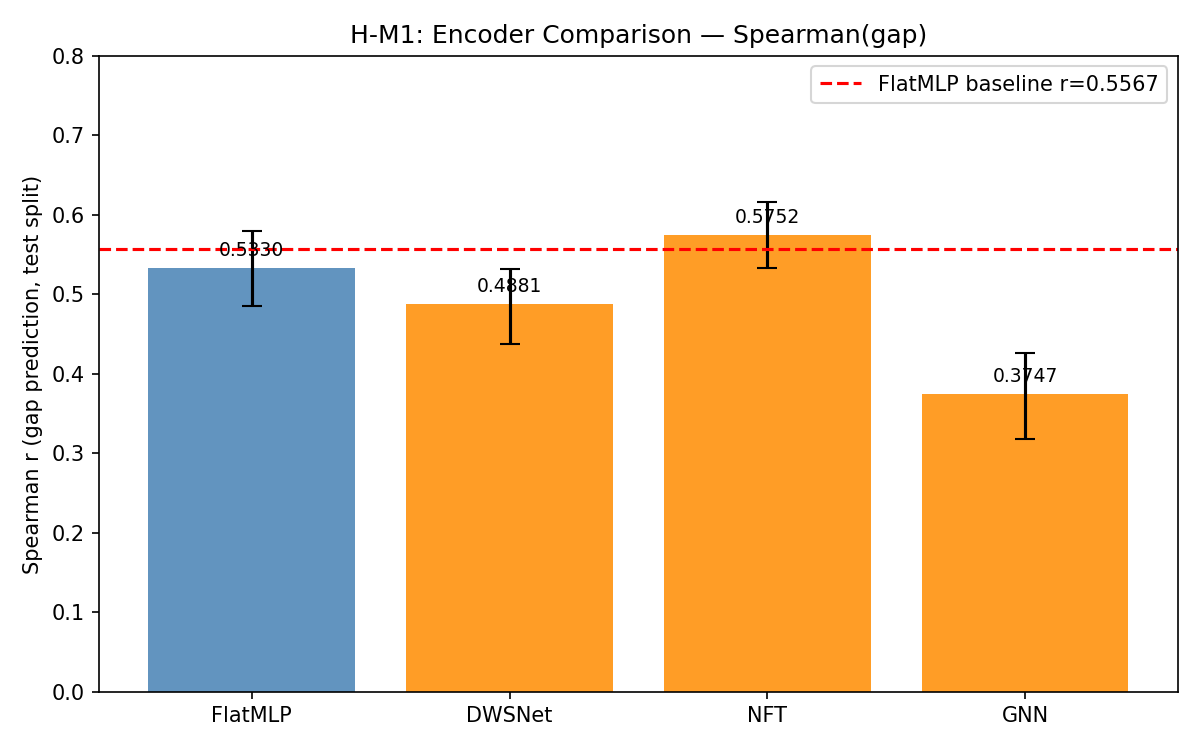
\includegraphics[width=\columnwidth]{figures/fig1_bar.png}
\caption{Spearman r per encoder on gap prediction with 95\% bootstrap CIs}
\label{fig:fig1_bar}
\end{figure}

\textbf{Figure 1.} Spearman rank correlation per encoder on gap prediction. Error bars are bootstrap 95\% CIs
(N = 1,000 resamples, seed 42). Horizontal reference line at FlatMLP r = 0.533. NFT is the only encoder
with a lower CI bound (0.534) exceeding FlatMLP's point estimate (0.533).

\begin{figure}[htbp]
\centering
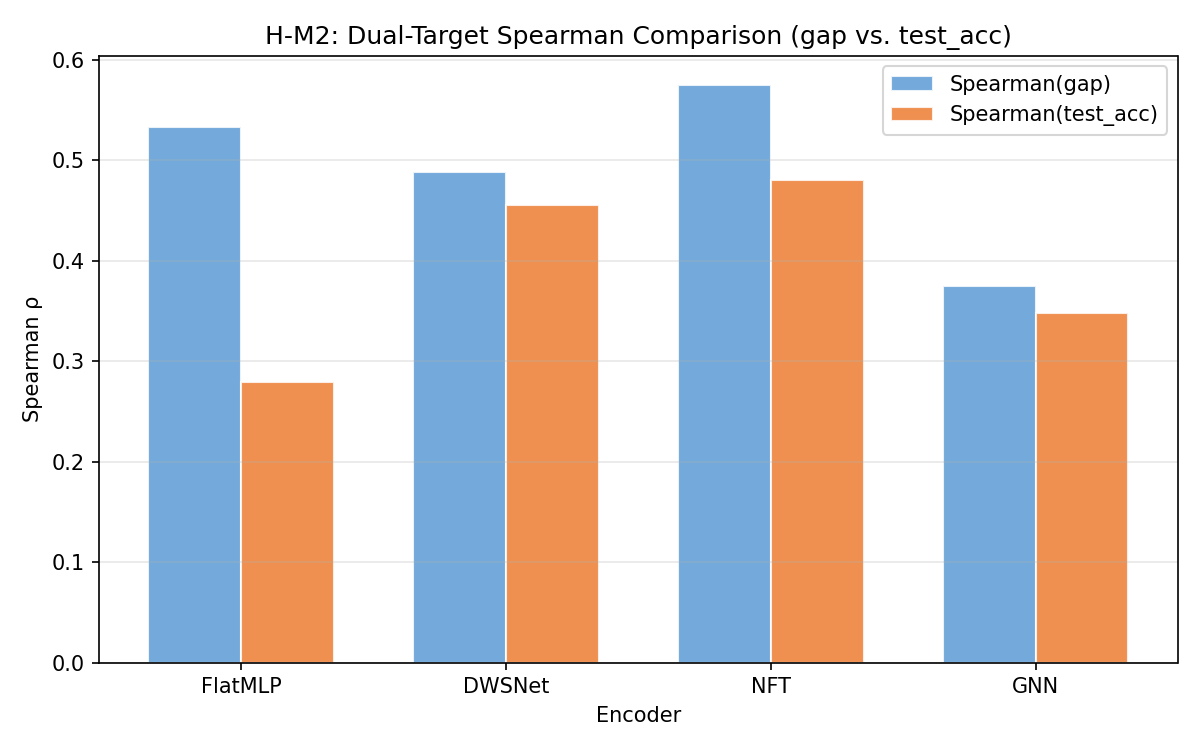
\includegraphics[width=\columnwidth]{figures/fig2_dual_target_spearman.png}
\caption{Side-by-side gap vs test\_acc Spearman for all four encoders}
\label{fig:fig2_dual_target_spearman}
\end{figure}

\textbf{Figure 2.} Dual-target Spearman comparison: all four encoders on both gap (primary) and test\_acc
(secondary). Reveals the gap > test\_acc asymmetry for FlatMLP (r = 0.533 vs. 0.279).

\begin{figure}[htbp]
\centering
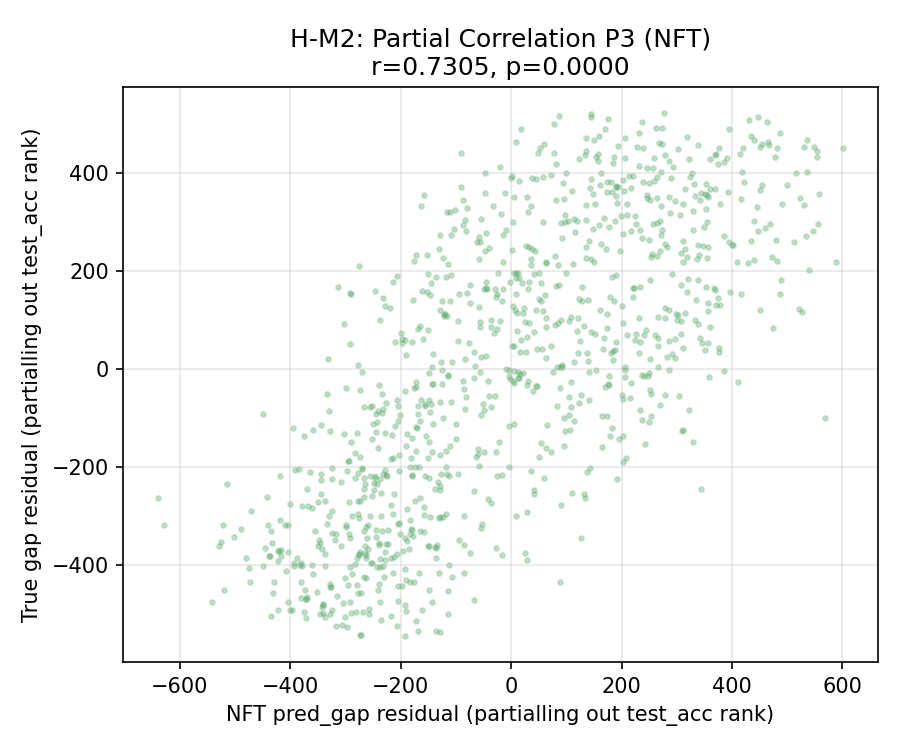
\includegraphics[width=\columnwidth]{figures/fig4_partial_corr_scatter.png}
\caption{NFT gap prediction residuals vs true gap residuals after partialling out test\_acc rank}
\label{fig:fig4_partial_corr_scatter}
\end{figure}

\textbf{Figure 3.} P3 partial Spearman scatter (rank residuals). X-axis: NFT gap prediction residuals after
regressing out test\_acc rank; Y-axis: true gap residuals after same regression. Partial Spearman r = 0.73
annotated; each point is one test-split model (N = 1,000).

\begin{figure}[htbp]
\centering
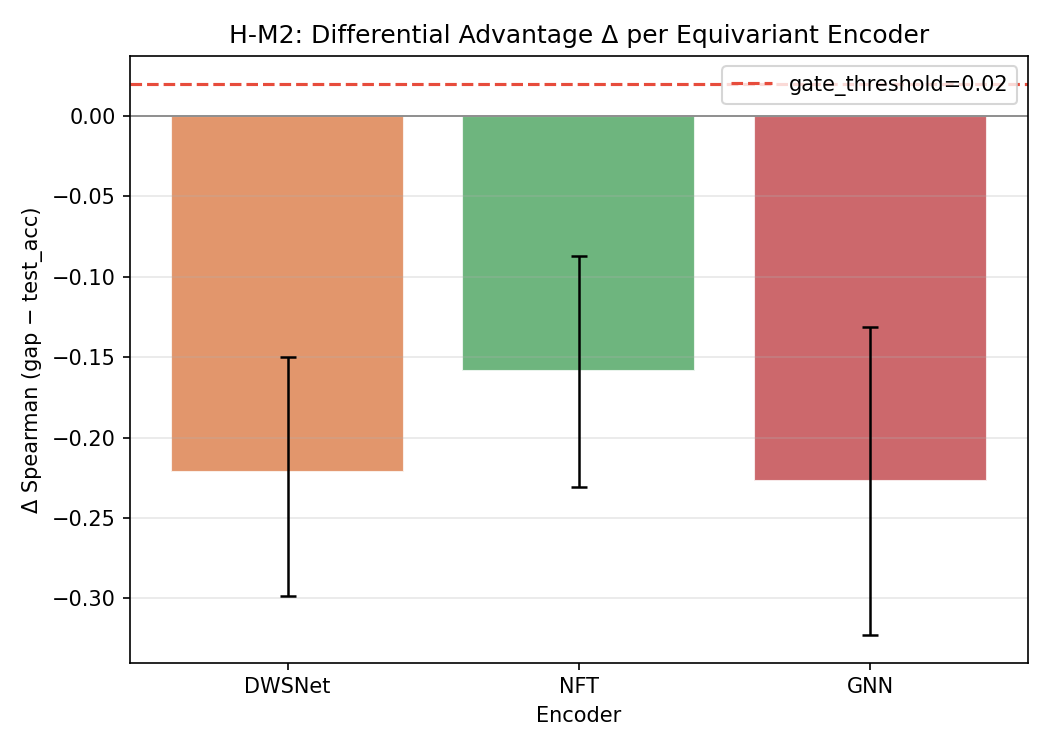
\includegraphics[width=\columnwidth]{figures/fig1_gate_delta.png}
\caption{Delta values for equivariant encoders with bootstrap 95\% CI and gate threshold}
\label{fig:fig1_gate_delta}
\end{figure}

\textbf{Figure 4.} Differential advantage $\Delta$ for equivariant encoders with 95\% bootstrap CI (horizontal
error bars) and gate threshold $\Delta$ = 0.02 (vertical reference line). All three $\Delta$ CIs lie entirely below
zero; gate criterion not met.

